% !TEX encoding = UTF-8 Unicode

\documentclass[twocolumn,10pt,a4j]{ltjsarticle}
\usepackage{kougai}
\setlength\intextsep{2mm}
\setlength\abovecaptionskip{2mm}

\title{Scratchからの移行を意識したプログラミング言語の開発}
\author{1932034 川原 史哉  指導教員 須田 宇宙 准教授}
\date{}

\begin{document}

\maketitle

\section{はじめに}
%背景
2020年度から小学校ではプログラミング教育の必修化が行われた.これに伴い,小学生でも扱いやすいビジュアルプログラミング言語が注目されている.
代表的なビジュアルプログラミング言語に「Scratch」がある.Scratchは指示の書かれたブロックを並べることで視覚的にわかりやすくプログラミングができる.そのため,初学者のプログラミング学習に適した教材となっている.

%世間の問題点
本格的なプログラムを作成していくうえで,テキストプログラミング言語の学習が必要になる.しかし,Scratchに慣れていると,テキストプログラミング言語の学習を始めようとしたときに仕様の違いから挫折してしまうことが問題点として挙げられる.例えば,スプライトの有無やソースコードの記述方法などが異なる.

%研究室内での問題点
当研究室では,上記の問題点を考慮したテキストプログラミング言語のインタープリタおよび実行環境の開発を行った.しかし,言語仕様がまとまっていない状況でインタープリタの開発を行なった結果,いくつかの不具合が生じてしまった\cite{senkou1}\cite{senkou2}.

%目的
そこで本研究では,先行研究で開発されたプログラミング言語「Chiba-lang」の言語仕様をまとめることを目的とする.

\section{先行研究}
先行研究では,ビジュアルプログラミングとテキストプログラミングについて調査を行い,初学者にもわかりやすいテキストプログラミング言語の基礎を示した\cite{senkou1}.また,その基礎をもとに,Scratchからの移行を考慮したテキストプログラミング言語のインタープリタおよび実行環境の開発を行った.しかし,言語仕様がまとまりきっておらず,いくつかの不具合が生じた.また,実行環境は実装には至らなかった\cite{senkou2}.

\section{Chiba-lang}
\subsection{コンセプト}
Scratchからテキストプログラミング言語への移行を考えたとき,「英語主体」や「スプライトが存在しない」などの相違点があり,学習者がプログラミングに対して苦手意識を持つ要因になる可能性がある.
そこで,Scratchからテキストプログラミング移行時の相違点などを考慮し,次のコンセプトを定めた.

\begin{enumerate}
   \item[(1)] Scratchと同様に,ステージ上でスプライトを動かすことができる.
   \item[(2)] 中学で学ぶ範囲の英単語や日常で使われるような英単語を使用する.
   \item[(3)] 上から下,左から右へと処理の流れがわかりやすい.
   \item[(4)] C言語におけるinclude文のような不要要素を排除する.
   \item[(5)] ブラウザ上での動作を前提とする.
\end{enumerate}

上記のコンセプトをもとに,言語仕様を定めた.

\subsection{記述サンプル}
\begin{figure}[h]
  \begin{minipage}[b]{0.5\linewidth}
    \centering
    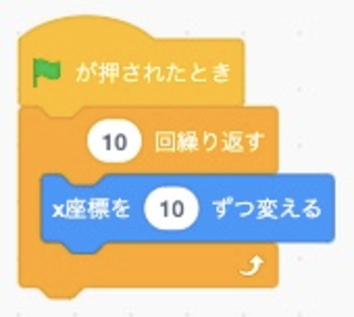
\includegraphics[scale=0.5]{figures/sample_scratch.pdf}
    \caption{Scratchの記述例}
    \label{fig:sample_scratch}
  \end{minipage}
  \begin{minipage}[b]{0.5\linewidth}
    \centering
    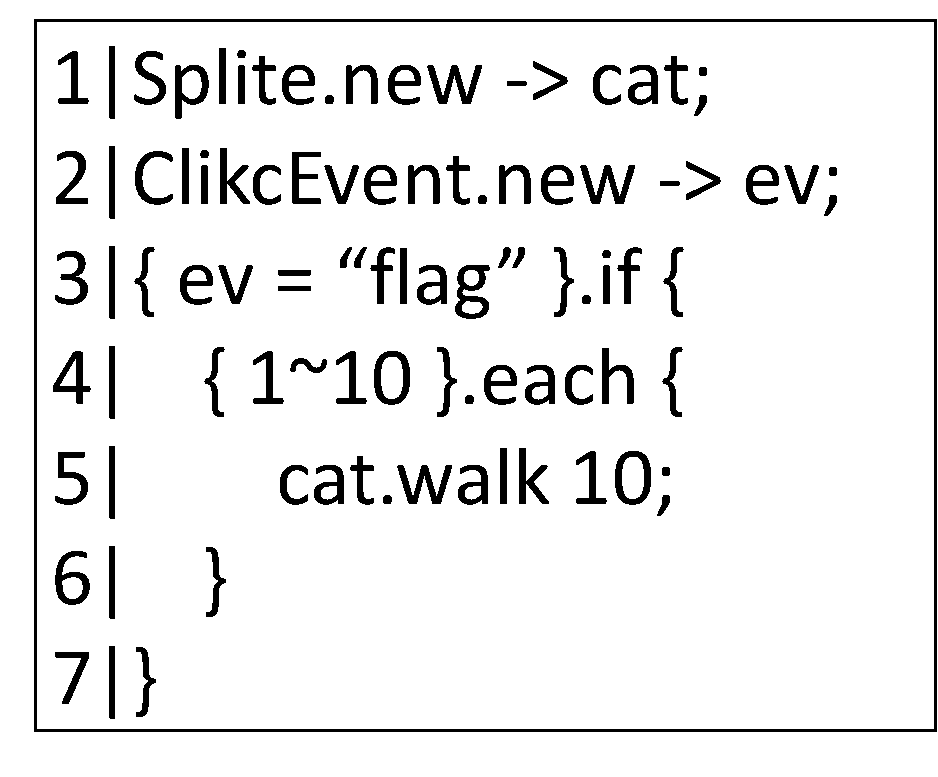
\includegraphics[scale=0.2]{figures/sample_chb.pdf}
    \caption{Chiba-langの記述例}
    \label{fig:sample_chb}
  \end{minipage}
\end{figure}

図\ref{fig:sample_scratch},\ref{fig:sample_chb}に,Scratchと本言語の記述例を示す.図\ref{fig:sample_scratch}と図\ref{fig:sample_chb}は同様の動作を行うソースコードである.これから図\ref{fig:sample_chb}をもとに説明していく.

Chiba-langでは,スプライトの動作やイベント処理などを司るクラスからインスタンスを作成することで,Scratchにおけるスプライトやイベントなどの機能を使うことができる.1行目,2行目でそれぞれスプライトを司るSpliteクラスとクリックに関連するイベントを司るClickEventクラスのインスタンスを作成している.

3行目では,図\ref{fig:sample_scratch}における「旗が押されとき」というイベントと同様の処理を表しており,evに"flag"というキーワードが送られときに中括弧内の処理を行う.

4行目では,図\ref{fig:sample_scratch}における「10回繰り返す」という制御と同様の処理を表しており,eachに範囲型の値を与えることで,その回数分の処理を繰り返す.テキスト言語におけるfor文と類似している.

5行目では,図\ref{fig:sample_scratch}における「x座標を10ずつ変える」という動きを行う.walkメソッドでx座標を10ずつ変更している.


\section{おわりに}
Scratchからの移行を意識したプログラミング言語「Chiba-lang」の言語仕様をまとめた.今後は,インタープリタおよび実行環境の開発を行う.

\begin{thebibliography}{99}
\bibitem{senkou1} 内掘美幸: ``Scratchからの移行を考慮したプログラミング言語と環境の開発'', 2019年度卒業研究
\bibitem{senkou2} 菅原直輝: ``Scratchからの移行を考慮したプログラミング言語の開発'', 2020年度卒業研究
\end{thebibliography}

\end{document}
